\section{Hitting-time derivations}
\label{app:hitting}

\paragraph{Complete graph.}
For $K_N$ with one marked vertex, every unmarked vertex is equivalent. Let $h$
be the expected hitting time from an unmarked vertex. Then
\begin{equation}
  h=1+\frac{N-2}{N-1}h,
\end{equation}
so $h=N-1$. Since the stationary distribution is uniform and we condition on
starting outside the marked set, $\HT=N-1$.

\paragraph{Cycle.}
For $C_N$ with marked vertex $0$, the expected hitting time from distance $i$ is
$h_i=i(N-i)$. It satisfies the recurrence
\begin{equation}
  h_i=1+\frac{1}{2}h_{i-1}+\frac{1}{2}h_{i+1},\qquad h_0=h_N=0,
\end{equation}
whose solution is the quadratic above. Averaging over
$i=1,\dots,N-1$ gives
\begin{equation}
  \HT=\frac{1}{N-1}\sum_{i=1}^{N-1}i(N-i)=\frac{N(N+1)}{6}.
\end{equation}
These identities are used as sanity checks in \texttt{tests/test\_classical.py}.

\section{Discriminant matrix and spectral identity}
\label{app:discriminant}

For a reversible chain, detailed balance gives
$\pi_xP_{xy}=\pi_yP_{yx}$, hence
\begin{equation}
  D_{xy}=\sqrt{P_{xy}P_{yx}}
  =\frac{\sqrt{\pi_x}P_{xy}}{\sqrt{\pi_y}},
\end{equation}
so $D=\mathrm{diag}(\pi)^{1/2}P\,\mathrm{diag}(\pi)^{-1/2}$. The matrices $D$
and $P$ are similar, so they have the same eigenvalues, and $D$ is symmetric.
The identity
\begin{equation}
  \langle\bar0|\langle x|W(P)|\bar0\rangle|y\rangle
  =\sqrt{P_{xy}P_{yx}}=D_{xy}
\end{equation}
follows directly from the definitions of $V(P)$, $\mathrm{Shift}$, and
$\mathrm{Ref}$. For the interpolated walk, the same computation gives the
top-left block $D(s)$, which is the starting point for the Chebyshev bound
\eqref{eq:chebyshev}.

\section{Measurement ensemble recursion}
\label{app:measurement}

Let $\lvert\phi_{x,a}\rangle=W(0)^a\lvert\bar0\rangle\lvert x\rangle$ for
$a=0,\dots,T_{\max}$, with position marginal
$\mu_{x,a}(y)=\lVert\Pi_y\lvert\phi_{x,a}\rangle\rVert^2$ and marked mass
$s_{x,a}=\sum_{y\in M}\mu_{x,a}(y)$. Let $\mu^{(0)}_a$ and $s^{(0)}_a$ be the
corresponding quantities for the initial state. A trajectory is described by
$q_0(t)$, the probability that no measurement has occurred by time $t$, and by
$q_{x,a}(t)$, the probability that the last reset was at vertex $x$ and the
state has evolved for $a$ steps since that reset.

At one step,
\begin{align}
  q_0(t+1)&=(1-p)q_0(t),\\
  q_{x,a+1}(t+1)&=(1-p)q_{x,a}(t),\\
  q_{y,1}(t+1)&=p\,q_0(t)\mu^{(0)}_t(y)
  +p\sum_{x,a}q_{x,a}(t)\mu_{x,a}(y).
\end{align}
The success probability is
\begin{equation}
  p_M(t+1)=q_0(t+1)s^{(0)}_{t+1}
  +\sum_{x,a}q_{x,a}(t+1)s_{x,a}.
\end{equation}
This recursion is exact for the channel \eqref{eq:measurement-channel}. It
requires the basis ensembles once per graph and marked set, after which a
sweep over $p$ is inexpensive. The implementation is in
\texttt{src/noise.py}.

For the detection model, the mass that a measurement places on $M$ is removed
instead of reset. With $f(t)$ the probability found by time $t$,
\begin{align}
  f(t+1)&=f(t)+p\sum_{y\in M}\Bigl[q_0(t)\mu^{(0)}_t(y)
  +\sum_{x,a}q_{x,a}(t)\mu_{x,a}(y)\Bigr],
\end{align}
the reset term $q_{y,1}(t+1)$ is restricted to $y\notin M$, and the probability
of having found the target with a final readout at $T$ is
$F_p(T)=f(T)+q_0(T)s^{(0)}_T+\sum_{x,a}q_{x,a}(T)s_{x,a}$.

\section{Additional results}
\label{app:additional}

\Cref{fig:e1-speedup} shows the classical-to-quantum speedup for E1. The cycle
has the largest speedup because its classical hitting time grows almost
quadratically; the complete graph has the smallest because its classical
hitting time grows only linearly.

\begin{figure}[t]
  \centering
  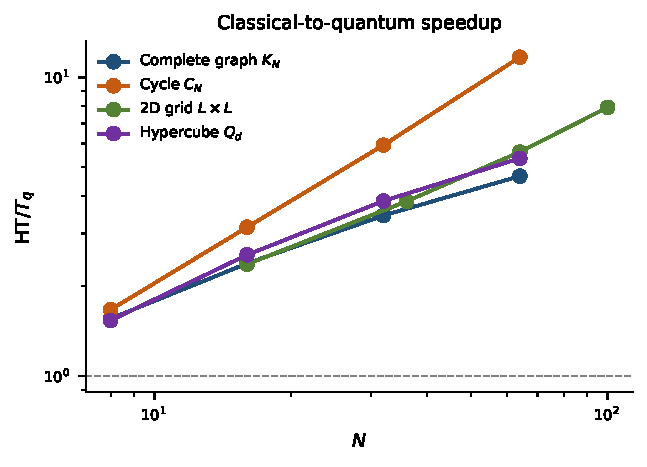
\includegraphics[width=0.72\linewidth]{figures/fig_e1_speedup.pdf}
  \caption{Classical-to-quantum speedup $\HT/T_q$ versus graph size for E1.}
  \label{fig:e1-speedup}
\end{figure}

\begin{table}[t]
  \centering
  \small
  \begin{tabular}{@{}llccccc@{}}
    \toprule
    Graph & Marked set & sets & median $\HT$ [min, max] & median $\HT^+/\HT$ & max $\HT^+/\HT$ & median $T_q$ \\
    \midrule
    Grid $6\times6$ & single & 1 & 46.1 & 1.00 & 1.00 & 12 \\
    Grid $6\times6$ & independent & 14 & 15.7 [12.7, 17.4] & 1.01 & 1.02 & 7 \\
    Grid $6\times6$ & clustered & 17 & 40.1 [17.6, 54.9] & 1.09 & 1.10 & 14 \\
    Grid $8\times8$ & single & 1 & 95.5 & 1.00 & 1.00 & 17 \\
    Grid $8\times8$ & independent & 18 & 34.8 [26.9, 39.7] & 1.02 & 1.05 & 10 \\
    Grid $8\times8$ & clustered & 18 & 85.0 [41.5, 131.1] & 1.06 & 1.09 & 20 \\
    Barbell $n=8$ & single & 1 & 373.6 & 1.00 & 1.00 & 51 \\
    Barbell $n=8$ & independent & 11 & 7.6 [7.1, 7.6] & 1.38 & 1.38 & 5 \\
    Barbell $n=8$ & clustered & 9 & 425.3 [196.6, 433.2] & 1.01 & 1.09 & 48 \\
    Barbell $n=16$ & single & 1 & 2558.0 & 1.00 & 1.00 & 134 \\
    Barbell $n=16$ & independent & 18 & 16.8 [16.4, 415.1] & 1.53 & 2.94 & 7 \\
    Barbell $n=16$ & clustered & 16 & 2768.0 [1893.1, 2781.3] & 1.00 & 1.04 & 133 \\
    \bottomrule
  \end{tabular}
  \caption{Full E2 results. Single targets have one set; other rows summarize
  all distinct sets from seeds $0,\dots,19$.}
  \label{tab:e2-full}
\end{table}

\section{Reproducibility}
\label{app:reproducibility}

The environment is created with
\begin{verbatim}
mamba env create -f environment.yml
mamba activate qwalk-cognition
\end{verbatim}
from \texttt{Final/code}. Everything is reproduced from \texttt{Final/code} with
\begin{verbatim}
make all
\end{verbatim}
which runs the tests, all six experiments, copies the figures used in the paper,
writes \texttt{results/MANIFEST.json} (git commit, dirty-tree flag, package
versions, and SHA-256 checksums of configs and results), and compiles the report.
Single experiments can be run with, for example,
\texttt{python -m src.experiments --only E6}. The complete run takes about
fifteen minutes, most of it in E4's robustness sweep. The test suite contains 71
passing tests. The configuration files are \texttt{configs/base.yaml} and
\texttt{configs/experiments.yaml}; all random choices use explicit seeds.
